\documentclass[twoside]{book}

% Packages required by doxygen
\usepackage{fixltx2e}
\usepackage{calc}
\usepackage{doxygen}
\usepackage[export]{adjustbox} % also loads graphicx
\usepackage{graphicx}
\usepackage[utf8]{inputenc}
\usepackage{makeidx}
\usepackage{multicol}
\usepackage{multirow}
\PassOptionsToPackage{warn}{textcomp}
\usepackage{textcomp}
\usepackage[nointegrals]{wasysym}
\usepackage[table]{xcolor}

% Font selection
\usepackage[T1]{fontenc}
\usepackage[scaled=.90]{helvet}
\usepackage{courier}
\usepackage{amssymb}
\usepackage{sectsty}
\renewcommand{\familydefault}{\sfdefault}
\allsectionsfont{%
  \fontseries{bc}\selectfont%
  \color{darkgray}%
}
\renewcommand{\DoxyLabelFont}{%
  \fontseries{bc}\selectfont%
  \color{darkgray}%
}
\newcommand{\+}{\discretionary{\mbox{\scriptsize$\hookleftarrow$}}{}{}}

% Page & text layout
\usepackage{geometry}
\geometry{%
  a4paper,%
  top=2.5cm,%
  bottom=2.5cm,%
  left=2.5cm,%
  right=2.5cm%
}
\tolerance=750
\hfuzz=15pt
\hbadness=750
\setlength{\emergencystretch}{15pt}
\setlength{\parindent}{0cm}
\setlength{\parskip}{3ex plus 2ex minus 2ex}
\makeatletter
\renewcommand{\paragraph}{%
  \@startsection{paragraph}{4}{0ex}{-1.0ex}{1.0ex}{%
    \normalfont\normalsize\bfseries\SS@parafont%
  }%
}
\renewcommand{\subparagraph}{%
  \@startsection{subparagraph}{5}{0ex}{-1.0ex}{1.0ex}{%
    \normalfont\normalsize\bfseries\SS@subparafont%
  }%
}
\makeatother

% Headers & footers
\usepackage{fancyhdr}
\pagestyle{fancyplain}
\fancyhead[LE]{\fancyplain{}{\bfseries\thepage}}
\fancyhead[CE]{\fancyplain{}{}}
\fancyhead[RE]{\fancyplain{}{\bfseries\leftmark}}
\fancyhead[LO]{\fancyplain{}{\bfseries\rightmark}}
\fancyhead[CO]{\fancyplain{}{}}
\fancyhead[RO]{\fancyplain{}{\bfseries\thepage}}
\fancyfoot[LE]{\fancyplain{}{}}
\fancyfoot[CE]{\fancyplain{}{}}
\fancyfoot[RE]{\fancyplain{}{\bfseries\scriptsize Generated by Doxygen }}
\fancyfoot[LO]{\fancyplain{}{\bfseries\scriptsize Generated by Doxygen }}
\fancyfoot[CO]{\fancyplain{}{}}
\fancyfoot[RO]{\fancyplain{}{}}
\renewcommand{\footrulewidth}{0.4pt}
\renewcommand{\chaptermark}[1]{%
  \markboth{#1}{}%
}
\renewcommand{\sectionmark}[1]{%
  \markright{\thesection\ #1}%
}

% Indices & bibliography
\usepackage{natbib}
\usepackage[titles]{tocloft}
\setcounter{tocdepth}{3}
\setcounter{secnumdepth}{5}
\makeindex

% Hyperlinks (required, but should be loaded last)
\usepackage{ifpdf}
\ifpdf
  \usepackage[pdftex,pagebackref=true]{hyperref}
\else
  \usepackage[ps2pdf,pagebackref=true]{hyperref}
\fi
\hypersetup{%
  colorlinks=true,%
  linkcolor=blue,%
  citecolor=blue,%
  unicode%
}

% Custom commands
\newcommand{\clearemptydoublepage}{%
  \newpage{\pagestyle{empty}\cleardoublepage}%
}

\usepackage{caption}
\captionsetup{labelsep=space,justification=centering,font={bf},singlelinecheck=off,skip=4pt,position=top}

%===== C O N T E N T S =====

\begin{document}

% Titlepage & ToC
\hypersetup{pageanchor=false,
             bookmarksnumbered=true,
             pdfencoding=unicode
            }
\pagenumbering{alph}
\begin{titlepage}
\vspace*{7cm}
\begin{center}%
{\Large C\+PP }\\
\vspace*{1cm}
{\large Generated by Doxygen 1.8.13}\\
\end{center}
\end{titlepage}
\clearemptydoublepage
\pagenumbering{roman}
\tableofcontents
\clearemptydoublepage
\pagenumbering{arabic}
\hypersetup{pageanchor=true}

%--- Begin generated contents ---
\chapter{Hierarchical Index}
\section{Class Hierarchy}
This inheritance list is sorted roughly, but not completely, alphabetically\+:\begin{DoxyCompactList}
\item \contentsline{section}{Figure}{\pageref{classFigure}}{}
\begin{DoxyCompactList}
\item \contentsline{section}{Disque}{\pageref{classDisque}}{}
\item \contentsline{section}{Rectangle}{\pageref{classRectangle}}{}
\item \contentsline{section}{Triangle}{\pageref{classTriangle}}{}
\end{DoxyCompactList}
\item \contentsline{section}{resultat}{\pageref{classresultat}}{}
\end{DoxyCompactList}

\chapter{Class Index}
\section{Class List}
Here are the classes, structs, unions and interfaces with brief descriptions\+:\begin{DoxyCompactList}
\item\contentsline{section}{\hyperlink{classDisque}{Disque} }{\pageref{classDisque}}{}
\item\contentsline{section}{\hyperlink{classFigure}{Figure} }{\pageref{classFigure}}{}
\item\contentsline{section}{\hyperlink{classRectangle}{Rectangle} }{\pageref{classRectangle}}{}
\item\contentsline{section}{\hyperlink{classresultat}{resultat} }{\pageref{classresultat}}{}
\item\contentsline{section}{\hyperlink{classTriangle}{Triangle} }{\pageref{classTriangle}}{}
\end{DoxyCompactList}

\chapter{File Index}
\section{File List}
Here is a list of all documented files with brief descriptions\+:\begin{DoxyCompactList}
\item\contentsline{section}{/root/figure/src/\hyperlink{disque_8h}{disque.\+h} }{\pageref{disque_8h}}{}
\item\contentsline{section}{/root/figure/src/\hyperlink{figure_8h}{figure.\+h} }{\pageref{figure_8h}}{}
\item\contentsline{section}{/root/figure/src/\hyperlink{rectangle_8h}{rectangle.\+h} }{\pageref{rectangle_8h}}{}
\item\contentsline{section}{/root/figure/src/\hyperlink{triangle_8h}{triangle.\+h} }{\pageref{triangle_8h}}{}
\end{DoxyCompactList}

\chapter{Class Documentation}
\hypertarget{classDisque}{}\section{Disque Class Reference}
\label{classDisque}\index{Disque@{Disque}}


Inheritance diagram for Disque\+:
\nopagebreak
\begin{figure}[H]
\begin{center}
\leavevmode
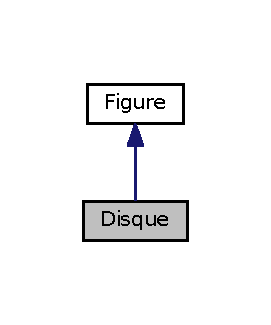
\includegraphics[width=130pt]{classDisque__inherit__graph}
\end{center}
\end{figure}


Collaboration diagram for Disque\+:
\nopagebreak
\begin{figure}[H]
\begin{center}
\leavevmode
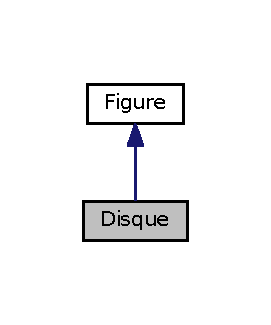
\includegraphics[width=130pt]{classDisque__coll__graph}
\end{center}
\end{figure}
\subsection*{Public Member Functions}
\begin{DoxyCompactItemize}
\item 
float \hyperlink{classDisque_a699609023203ea173b117df83f5c55bd}{calcul\+Perimetre} (float a)
\item 
float \hyperlink{classDisque_a6a721908949195bc8c8c0388c034b30a}{calcul\+Surface} (float a)
\end{DoxyCompactItemize}
\subsection*{Public Attributes}
\begin{DoxyCompactItemize}
\item 
\mbox{\Hypertarget{classDisque_a50ee9a093fd89c4519ca9a782f0161de}\label{classDisque_a50ee9a093fd89c4519ca9a782f0161de}} 
float {\bfseries rayon}
\end{DoxyCompactItemize}


\subsection{Member Function Documentation}
\mbox{\Hypertarget{classDisque_a699609023203ea173b117df83f5c55bd}\label{classDisque_a699609023203ea173b117df83f5c55bd}} 
\index{Disque@{Disque}!calcul\+Perimetre@{calcul\+Perimetre}}
\index{calcul\+Perimetre@{calcul\+Perimetre}!Disque@{Disque}}
\subsubsection{\texorpdfstring{calcul\+Perimetre()}{calculPerimetre()}}
{\footnotesize\ttfamily float Disque\+::calcul\+Perimetre (\begin{DoxyParamCaption}\item[{float}]{a }\end{DoxyParamCaption})}

param calcul\+Perimetre va calculer le perimetre d\textquotesingle{}un disque ou cercle \mbox{\Hypertarget{classDisque_a6a721908949195bc8c8c0388c034b30a}\label{classDisque_a6a721908949195bc8c8c0388c034b30a}} 
\index{Disque@{Disque}!calcul\+Surface@{calcul\+Surface}}
\index{calcul\+Surface@{calcul\+Surface}!Disque@{Disque}}
\subsubsection{\texorpdfstring{calcul\+Surface()}{calculSurface()}}
{\footnotesize\ttfamily float Disque\+::calcul\+Surface (\begin{DoxyParamCaption}\item[{float}]{a }\end{DoxyParamCaption})}

param calcul\+Surface va calculer la surface d\textquotesingle{}un disque ou cercle 

The documentation for this class was generated from the following files\+:\begin{DoxyCompactItemize}
\item 
/root/figure/src/\hyperlink{disque_8h}{disque.\+h}\item 
/root/figure/src/disque.\+cpp\end{DoxyCompactItemize}

\hypertarget{classFigure}{}\section{Figure Class Reference}
\label{classFigure}\index{Figure@{Figure}}


Inheritance diagram for Figure\+:
\nopagebreak
\begin{figure}[H]
\begin{center}
\leavevmode
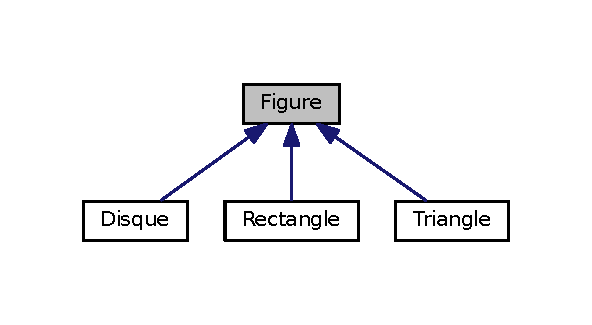
\includegraphics[width=284pt]{classFigure__inherit__graph}
\end{center}
\end{figure}
\subsection*{Public Member Functions}
\begin{DoxyCompactItemize}
\item 
virtual float \hyperlink{classFigure_aa099ec99ff69eb0e4f989af6a8ea9350}{calcul\+Surface} ()
\item 
virtual int \hyperlink{classFigure_aa44c45980a77a4ffd8f37a2ef88c747f}{calcul\+Perimetre} ()
\end{DoxyCompactItemize}


\subsection{Member Function Documentation}
\mbox{\Hypertarget{classFigure_aa44c45980a77a4ffd8f37a2ef88c747f}\label{classFigure_aa44c45980a77a4ffd8f37a2ef88c747f}} 
\index{Figure@{Figure}!calcul\+Perimetre@{calcul\+Perimetre}}
\index{calcul\+Perimetre@{calcul\+Perimetre}!Figure@{Figure}}
\subsubsection{\texorpdfstring{calcul\+Perimetre()}{calculPerimetre()}}
{\footnotesize\ttfamily int Figure\+::calcul\+Perimetre (\begin{DoxyParamCaption}{ }\end{DoxyParamCaption})\hspace{0.3cm}{\ttfamily [virtual]}}

param calcul\+Perimetre va être définit dans les classes enfant \mbox{\Hypertarget{classFigure_aa099ec99ff69eb0e4f989af6a8ea9350}\label{classFigure_aa099ec99ff69eb0e4f989af6a8ea9350}} 
\index{Figure@{Figure}!calcul\+Surface@{calcul\+Surface}}
\index{calcul\+Surface@{calcul\+Surface}!Figure@{Figure}}
\subsubsection{\texorpdfstring{calcul\+Surface()}{calculSurface()}}
{\footnotesize\ttfamily float Figure\+::calcul\+Surface (\begin{DoxyParamCaption}{ }\end{DoxyParamCaption})\hspace{0.3cm}{\ttfamily [virtual]}}

param calcul\+Surface va être définit dans les classes enfant 

The documentation for this class was generated from the following files\+:\begin{DoxyCompactItemize}
\item 
/root/figure/src/\hyperlink{figure_8h}{figure.\+h}\item 
/root/figure/src/figure.\+cpp\end{DoxyCompactItemize}

\hypertarget{classRectangle}{}\section{Rectangle Class Reference}
\label{classRectangle}\index{Rectangle@{Rectangle}}


Inheritance diagram for Rectangle\+:
\nopagebreak
\begin{figure}[H]
\begin{center}
\leavevmode
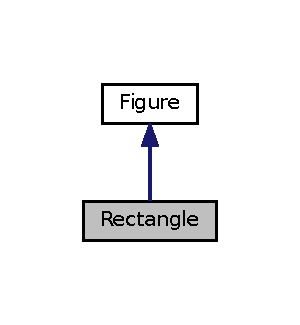
\includegraphics[width=144pt]{classRectangle__inherit__graph}
\end{center}
\end{figure}


Collaboration diagram for Rectangle\+:
\nopagebreak
\begin{figure}[H]
\begin{center}
\leavevmode
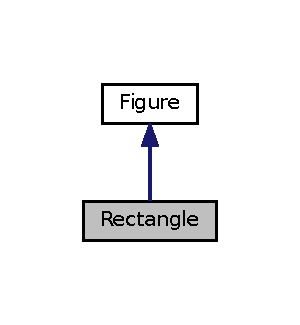
\includegraphics[width=144pt]{classRectangle__coll__graph}
\end{center}
\end{figure}
\subsection*{Public Member Functions}
\begin{DoxyCompactItemize}
\item 
float \hyperlink{classRectangle_a2931c93ead4aa6ac3e337de151dcd49c}{calcul\+Surface} (float a, float b)
\item 
float \hyperlink{classRectangle_aa90f2be32fb070a870405842ec55c1be}{calcul\+Perimetre} (float a, float b)
\end{DoxyCompactItemize}
\subsection*{Public Attributes}
\begin{DoxyCompactItemize}
\item 
\mbox{\Hypertarget{classRectangle_aea28f8e235d7d8c79dc53d5436c0bc85}\label{classRectangle_aea28f8e235d7d8c79dc53d5436c0bc85}} 
float {\bfseries longueur}
\item 
\mbox{\Hypertarget{classRectangle_a66e10016113076e07fa361871b82d819}\label{classRectangle_a66e10016113076e07fa361871b82d819}} 
float {\bfseries largeur}
\end{DoxyCompactItemize}


\subsection{Member Function Documentation}
\mbox{\Hypertarget{classRectangle_aa90f2be32fb070a870405842ec55c1be}\label{classRectangle_aa90f2be32fb070a870405842ec55c1be}} 
\index{Rectangle@{Rectangle}!calcul\+Perimetre@{calcul\+Perimetre}}
\index{calcul\+Perimetre@{calcul\+Perimetre}!Rectangle@{Rectangle}}
\subsubsection{\texorpdfstring{calcul\+Perimetre()}{calculPerimetre()}}
{\footnotesize\ttfamily float Rectangle\+::calcul\+Perimetre (\begin{DoxyParamCaption}\item[{float}]{a,  }\item[{float}]{b }\end{DoxyParamCaption})}

calcule le perimetre d\textquotesingle{}un rectangle \mbox{\Hypertarget{classRectangle_a2931c93ead4aa6ac3e337de151dcd49c}\label{classRectangle_a2931c93ead4aa6ac3e337de151dcd49c}} 
\index{Rectangle@{Rectangle}!calcul\+Surface@{calcul\+Surface}}
\index{calcul\+Surface@{calcul\+Surface}!Rectangle@{Rectangle}}
\subsubsection{\texorpdfstring{calcul\+Surface()}{calculSurface()}}
{\footnotesize\ttfamily float Rectangle\+::calcul\+Surface (\begin{DoxyParamCaption}\item[{float}]{a,  }\item[{float}]{b }\end{DoxyParamCaption})}

calcule la surface d\textquotesingle{}un rectangle 

The documentation for this class was generated from the following files\+:\begin{DoxyCompactItemize}
\item 
/root/figure/src/\hyperlink{rectangle_8h}{rectangle.\+h}\item 
/root/figure/src/rectangle.\+cpp\end{DoxyCompactItemize}

\hypertarget{classresultat}{}\section{resultat Class Reference}
\label{classresultat}\index{resultat@{resultat}}


{\ttfamily \#include $<$figure.\+h$>$}



\subsection{Detailed Description}
classe va servir pour définir après la classe pour chaque enfant 

The documentation for this class was generated from the following file\+:\begin{DoxyCompactItemize}
\item 
/root/figure/src/\hyperlink{figure_8h}{figure.\+h}\end{DoxyCompactItemize}

\hypertarget{classTriangle}{}\section{Triangle Class Reference}
\label{classTriangle}\index{Triangle@{Triangle}}


{\ttfamily \#include $<$triangle.\+h$>$}



Inheritance diagram for Triangle\+:
\nopagebreak
\begin{figure}[H]
\begin{center}
\leavevmode
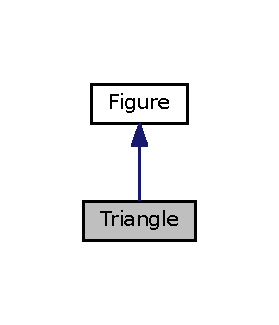
\includegraphics[width=134pt]{classTriangle__inherit__graph}
\end{center}
\end{figure}


Collaboration diagram for Triangle\+:
\nopagebreak
\begin{figure}[H]
\begin{center}
\leavevmode
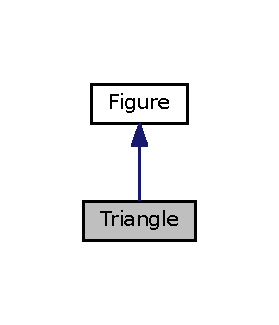
\includegraphics[width=134pt]{classTriangle__coll__graph}
\end{center}
\end{figure}
\subsection*{Public Member Functions}
\begin{DoxyCompactItemize}
\item 
float \hyperlink{classTriangle_afeb2eb1920e4a0d0f376c32b7797e766}{calcul\+Perimetre} (float a, float b, float c)
\item 
float \hyperlink{classTriangle_abf1ce3d4215d2f66f7030a569634a40a}{calcul\+Surface} (float a, float d)
\end{DoxyCompactItemize}
\subsection*{Public Attributes}
\begin{DoxyCompactItemize}
\item 
\mbox{\Hypertarget{classTriangle_a11345292059387564112d3b7267bfad5}\label{classTriangle_a11345292059387564112d3b7267bfad5}} 
float {\bfseries cote1}
\item 
\mbox{\Hypertarget{classTriangle_a5111045d46caaac8295a17ef499d4e75}\label{classTriangle_a5111045d46caaac8295a17ef499d4e75}} 
float {\bfseries cote2}
\item 
\mbox{\Hypertarget{classTriangle_a9d7c379bf68c5bf62461de936dc5776b}\label{classTriangle_a9d7c379bf68c5bf62461de936dc5776b}} 
float {\bfseries cote3}
\item 
\mbox{\Hypertarget{classTriangle_a329b79974da202a0bba86ba1f6ce0a96}\label{classTriangle_a329b79974da202a0bba86ba1f6ce0a96}} 
float {\bfseries hauteur}
\end{DoxyCompactItemize}


\subsection{Detailed Description}
qui calcule surface et perimetre d\textquotesingle{}un triangle 

\subsection{Member Function Documentation}
\mbox{\Hypertarget{classTriangle_afeb2eb1920e4a0d0f376c32b7797e766}\label{classTriangle_afeb2eb1920e4a0d0f376c32b7797e766}} 
\index{Triangle@{Triangle}!calcul\+Perimetre@{calcul\+Perimetre}}
\index{calcul\+Perimetre@{calcul\+Perimetre}!Triangle@{Triangle}}
\subsubsection{\texorpdfstring{calcul\+Perimetre()}{calculPerimetre()}}
{\footnotesize\ttfamily float Triangle\+::calcul\+Perimetre (\begin{DoxyParamCaption}\item[{float}]{a,  }\item[{float}]{b,  }\item[{float}]{c }\end{DoxyParamCaption})}

param calcul\+Perimetre ici va calculer le perimetre du triangle \mbox{\Hypertarget{classTriangle_abf1ce3d4215d2f66f7030a569634a40a}\label{classTriangle_abf1ce3d4215d2f66f7030a569634a40a}} 
\index{Triangle@{Triangle}!calcul\+Surface@{calcul\+Surface}}
\index{calcul\+Surface@{calcul\+Surface}!Triangle@{Triangle}}
\subsubsection{\texorpdfstring{calcul\+Surface()}{calculSurface()}}
{\footnotesize\ttfamily float Triangle\+::calcul\+Surface (\begin{DoxyParamCaption}\item[{float}]{a,  }\item[{float}]{d }\end{DoxyParamCaption})}

param calcul\+Surface ici va calculer la surface du triangle 

The documentation for this class was generated from the following files\+:\begin{DoxyCompactItemize}
\item 
/root/figure/src/\hyperlink{triangle_8h}{triangle.\+h}\item 
/root/figure/src/triangle.\+cpp\end{DoxyCompactItemize}

\chapter{File Documentation}
\hypertarget{disque_8h}{}\section{/root/figure/src/disque.h File Reference}
\label{disque_8h}\index{/root/figure/src/disque.\+h@{/root/figure/src/disque.\+h}}
{\ttfamily \#include \char`\"{}figure.\+h\char`\"{}}\newline
{\ttfamily \#include $<$iostream$>$}\newline
Include dependency graph for disque.\+h\+:
\nopagebreak
\begin{figure}[H]
\begin{center}
\leavevmode
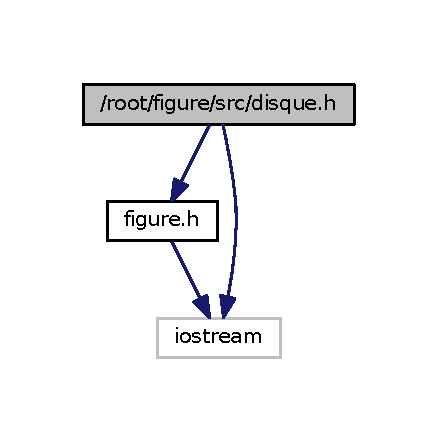
\includegraphics[width=210pt]{disque_8h__incl}
\end{center}
\end{figure}
\subsection*{Classes}
\begin{DoxyCompactItemize}
\item 
class \hyperlink{classDisque}{Disque}
\end{DoxyCompactItemize}


\subsection{Detailed Description}
de la classe disque  Maudet version 1.\+0 
\hypertarget{figure_8h}{}\section{/root/figure/src/figure.h File Reference}
\label{figure_8h}\index{/root/figure/src/figure.\+h@{/root/figure/src/figure.\+h}}
{\ttfamily \#include $<$iostream$>$}\newline
Include dependency graph for figure.\+h\+:
\nopagebreak
\begin{figure}[H]
\begin{center}
\leavevmode
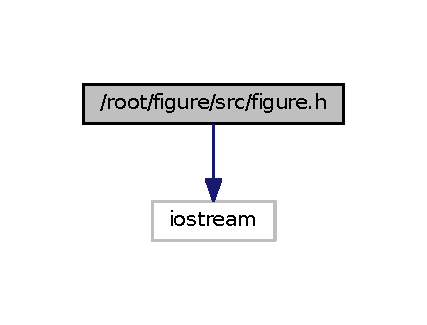
\includegraphics[width=205pt]{figure_8h__incl}
\end{center}
\end{figure}
This graph shows which files directly or indirectly include this file\+:
\nopagebreak
\begin{figure}[H]
\begin{center}
\leavevmode
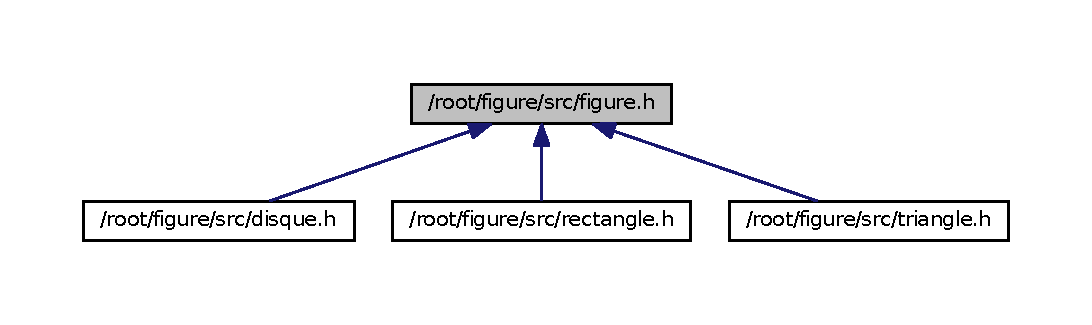
\includegraphics[width=350pt]{figure_8h__dep__incl}
\end{center}
\end{figure}
\subsection*{Classes}
\begin{DoxyCompactItemize}
\item 
class \hyperlink{classFigure}{Figure}
\end{DoxyCompactItemize}


\subsection{Detailed Description}
parent de disque, rectangle et triangle  Maudet version 1.\+0 
\hypertarget{rectangle_8h}{}\section{/root/figure/src/rectangle.h File Reference}
\label{rectangle_8h}\index{/root/figure/src/rectangle.\+h@{/root/figure/src/rectangle.\+h}}
{\ttfamily \#include \char`\"{}figure.\+h\char`\"{}}\newline
{\ttfamily \#include $<$iostream$>$}\newline
Include dependency graph for rectangle.\+h\+:
\nopagebreak
\begin{figure}[H]
\begin{center}
\leavevmode
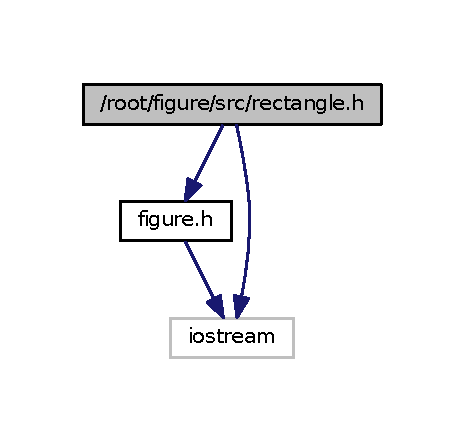
\includegraphics[width=223pt]{rectangle_8h__incl}
\end{center}
\end{figure}
\subsection*{Classes}
\begin{DoxyCompactItemize}
\item 
class \hyperlink{classRectangle}{Rectangle}
\end{DoxyCompactItemize}


\subsection{Detailed Description}
éfinition de la classe rectangle  Maudet version 1.\+0 
\hypertarget{triangle_8h}{}\section{/root/figure/src/triangle.h File Reference}
\label{triangle_8h}\index{/root/figure/src/triangle.\+h@{/root/figure/src/triangle.\+h}}
{\ttfamily \#include \char`\"{}figure.\+h\char`\"{}}\newline
Include dependency graph for triangle.\+h\+:
\nopagebreak
\begin{figure}[H]
\begin{center}
\leavevmode
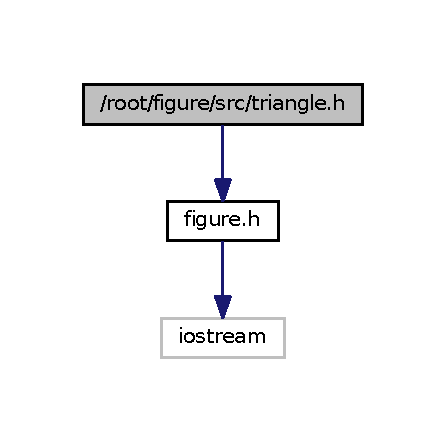
\includegraphics[width=214pt]{triangle_8h__incl}
\end{center}
\end{figure}
\subsection*{Classes}
\begin{DoxyCompactItemize}
\item 
class \hyperlink{classTriangle}{Triangle}
\end{DoxyCompactItemize}


\subsection{Detailed Description}
éfinition de la classe triangle  Maudet version 1.\+0 
%--- End generated contents ---

% Index
\backmatter
\newpage
\phantomsection
\clearemptydoublepage
\addcontentsline{toc}{chapter}{Index}
\printindex

\end{document}
